\chapter{Methods and tools: regional simulations with the IPSL Climate Model}
\label{chap:methods}
\minitoc
\pagebreak

This work uses the atmosphere and land surface components of the IPSL-CM, which has been a regular participant in CMIP exercises, including CMIP6 \citep{boucher_presentation_2020}. 

\section{ICOLMDZ atmospheric model}
\subsection{Dynamical core and parameterizations}
The atmospheric component of the model is the association of the dynamical core DYNAMICO \citep{dubos_dynamico-10_2015}, and the LMDZ6A physics used for CMIP6 \citep{hourdin_lmdz6a_2020}. 

Icosahedral dynamical cores already existed in some models, such as ICON \citep{zangl_icon_2015,giorgetta_icon-_2018,prill_icon_nodate}
%todo: màj prill2022
, and was introduced in the IPSL-CM with the main objective of standardizing grid cells for global simulations. In particular, it avoids the discrepancies of a "regular" longitude-latitude grid that appear at the poles, opening new prospects for modeling projects in the Arctic %todo:cite project ?
and Antarctic regions. %todo:cite AWACA ?
All simulations run in the thesis used a 30s time step for the dynamics.

The physics of the model are version NPv6.2 with 79 vertical levels, and are run every 15 mn.
They include the following parameterizations:
\begin{itemize}
    \item a surface layer description based on \cite{louis_parametric_1979} and \cite{king_sensitivity_2001}; 
    %option: give more details into ATKE scheme and consequences for surface layer ? not used here but...
    \item an Eddy-Diffusivity Mass Flux (EDMF) scheme of boundary layer vertical transfer composed of a turbulent diffusion scheme based on \cite{yamada_simulations_1983} with recent improvements described in \cite{vignon_modeling_2018}, and a thermal plume model for shallow convection \citep{rio_thermal_2008, hourdin_unified_2019}; 
    \item a mass-flux scheme for deep convection based on Emanuel's scheme \citep{emanuel_scheme_1991, grandpeix_improved_2004, rio_control_2013}, with stochastic triggering \citep{rochetin_deep_2014, rochetin_deep_2014-1}; 
    \item a parameterization of the cold pools created below cumulonimbus by reevaporation of convective rainfall \citep{grandpeix_density_2010-1,grandpeix_density_2010};
    \item a large scale condensation scheme based on a statistical distribution of subgrid total water content, from which cloud fraction and water contents are derived \citep{madeleine_improved_2020}; 
    \item radiative transfer model RRTM \citep{mlawer_radiative_1997}.
\end{itemize}

%todo:detail forcings : solar, SST ans SIC from AMIP -> ref ? (thèse Pedro ?)
All simulations were run with prescribed sea surface temperature and sea ice content from the AMIP dataset.

\subsection{Limited area model configuration}
Simulations are run in a limited area model (LAM) configuration, first used and described in \citet{raillard_leveraging_2024}. It must be noted that the use of this model in the IPSL community is very recent, that it is still evolving quickly, and that its evaluation is still ongoing. In particular, the simulations presented in chapter \ref{chap:monthly} constitute the first case study focusing on the water cycle and land-atmosphere interactions, as well as the first use case at the midlatitudes.

\subsubsection{Boundary conditions}
Since simulations with the LAM only cover a portion of the globe, lateral boundary conditions are read by the model from a forcing file, which can be obtained from various sources. 
In most of the work presented here, lateral boundary conditions for the LAM were taken from ERA5 reanalysis hourly values at 0.25° resolution \citep{hersbach_era5_2020}.  This product uses a model with observation data assimilation techniques to produce outputs that are as close as possible to actual conditions. When simulating recent climate, using this forcing enables having rather realistic synoptic conditions. 
It is also possible to run the model with other sources for the forcing file, in particular using outputs from global climate simulations, either from the ICOLMDZ global model or from other models. The modelling community at IPSL is also currently investigating the possibility of using mean outputs from the CMIP6 simulations under various SSPs to run the LAM in possible future climate conditions.

To run a regional simulation, the forcing file must contain data for the nudged variables %todo:confirm if CIWC and CLWC
as well as some other variables at the surface that are used to manage initialization. %todo:clarify

\begin{table}[htbp]
\centering
\begin{tabular}{|l|l|}
\hline
\multicolumn{2}{|c|}{\textbf{Variables on vertical levels}} \\ \hline
Air temperature                & t     \\ \hline
Zonal wind                    & u     \\ \hline
Meridional wind               & v     \\ \hline
Relative humidity             & r     \\ \hline
Specific humidity             & q     \\ \hline
Specific liquid water content & clwc  \\ \hline
Specific ice water content    & ciwc  \\ \hline
\multicolumn{2}{|c|}{\textbf{Surface variables}} \\ \hline
2m air temperature            & t2m   \\ \hline
Surface geopotential          & z     \\ \hline
Surface pressure              & p     \\ \hline
\end{tabular}
\caption{List of variables required in the LAM forcing file.}
\end{table}

%option:explain init ? orography ?


\subsubsection{Domain structure and nudging method}

The simulation domain is a large hexagon composed of hexagonal grid cells, and defined by three parameters:
\begin{itemize}
    \item The centre of the hexagon (latitude and longitude).
    \item The radius of hexagon, distance between the centre and one of the vertices, in kilometers.
    \item The number of grid cells on this radius, referred to as NBP.
\end{itemize}

The resolution of the model (diameter of one grid cell) is directly obtained by dividing the radius by the NBP.

\hfill

The simulation domain is separated in 3 concentric zones, as shown on Fig. \ref{fig:LAM_domain}: 
\begin{itemize}
    \item The raw forcing zone which contains values directly given by the forcing, consisting of 5 grid cells.
    \item The transition zone  where the model is nudged toward the forcing with decreasing strength, consisting of 8 grid cells.
    \item the free zone at the centre of the domain where there is no direct influence of the lateral forcing, with all the remaining grid cells (NBP - 8 - 5).
\end{itemize} 

\begin{figure}[ht]
    \centering
    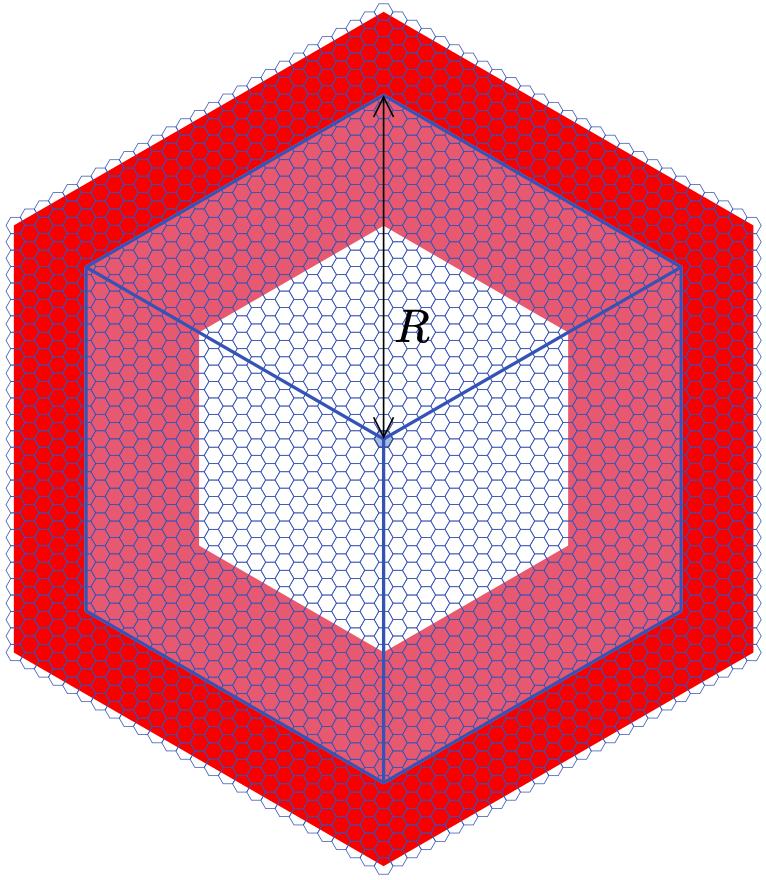
\includegraphics[width=0.5\linewidth]{images/LAM_domain_zones.png}
    \caption{LAM domain structure example with NBP=27 \citep[from][]{raillard_leveraging_2024}}
    \label{fig:LAM_domain}
\end{figure}

The concept of nudging are well known in climate modelling and NWP, since it is often used to manage boundary conditions in regional models, or to reproduce realistic situations for comparison to observations or to study specific events. Nudging is done by adding a forcing term in the equation that governs the evolution of a given prognostic variable V in the model, to drive it towards a reference value $V_{ref}$ over a given time scale $\tau$.
. %tocheck : prognostic only ? how do we use CIWC, CLWC then ?(or maybe they are prognostic too ?)

\begin{equation}
    \frac{\partial V}{\partial t} = \frac{\partial V}{\partial t}_{\text{model}}+ \frac{V_{\text{ref}} - V}{\tau}
\end{equation}

The strength of the nudging can be modulated by adjusting the time scale $\tau$.
In the raw forcing zone, $\tau = 3600s$ and in the free zone, $\tau$ is infinite, meaning the forcing term does not alter the equation. In the transition zone inbetween, the value of $\tau$ is gradually increased over the 8 grid cells, following an arctan profile, to smooth the transition.

Nudging is applied at every time step of the dynamics (30s here). The reference value for each variable is obtained by temporally interpolating the forcing file to this time step. The sampling frequency of the forcing file can have an impact on the simulation. In this work, hourly forcing files were used for most of the simulations, but some sensitivity experiments were made using forcing data sampled every six hours.

\subsubsection{Technical specificities}

While running the first simulations with the LAM, various occurrences of inappropriate model behaviour were observed at the top of the atmosphere, reaching temperatures over 373K. Based on prior expereience of the model developper, this was attributed to inconsistent quantities of air in these layers of very low density, which could lead to excessive heating over one model time step. The unusual interaction of advection from the dynamics and nudging were thought to be responsible for anomalies in the matter and energy budgets, in or near the transition zone.
To solve this issue, an additionnal nudging of temperature and wind components was applied for the upper layers of the atmosphere (above 1hPa) over the whole domain, to ensure that values remaines in a reasonible order of magnitude. 

\hfill

On a different topic, it must also be noted that the model computes all variables on its hexagonal grid cells. However, it is not very straightfroward to analyse and display simulation data on such a grid since most usual tools (ferret, ncview, matplotlib) struggle with the coordinates system. 
By default, LAM outputs are therefore interpolated to a regular longitude-latitude grid, but can be obtained on the native hexagonal grid if needed.
In this work, the simulations used in Chapter \ref{chap:monthly} were analysed solely using the interpolated outputs, while simulations used in Chapter \ref{chap:liaise}, which used specific grid cells for comparison to observation, were analysed using the native hexagonal grid.

%option:discuss choice of domain (100 vs 1500 vs 2000km ?)

\section{ORCHIDEE land surface model}
\subsection{General structure, running modes, and input data}
ORCHIDEE (Organizing Carbon and Hydrology In Dynamic EcosystEms) is a land surface model. Various "branches" and versions exist within the model, as the base structure presented in \citet{krinner_dynamic_2005} has been adapted and extended to meet different research objectives. 
This work uses branch 2.2 \citep{cheruy_improved_2020}, which served as the land component of the IPSL climate model for CMIP6 simulations \citep{boucher_presentation_2020}. While the version chosen for CMIP7 simulations is ORCHIDEE v.4.2, which integrates recent developments for the modeling of snow, permafrost, vegetation, carbon, nitrogen and phosphorus cycles %todo:check, add major other elements 
, branch 2.2 is still used for development focused on surface hydrology, that can then be introduced in other branches.
%Coupling with an atmosphere and ocean model imposes significant computational constraints, leading to the simplification or omission of certain processes for global climate simulations.
The description of this model version provided here is partly based on Section 2 of Aurélien Campoy’s PhD thesis \citep{campoy_influence_2013}. %todo:check si j'ai le droit de faire/dire ça...

ORCHIDEE v2.2 includes several modules:
\begin{itemize}
    \item SECHIBA (\textit{Schématisation des Échanges Hydriques à l’Interface entre la Biosphère et l’Atmosphère}, \cite{ducoudre_sechiba_1993}). Initially integrated into the surface scheme of the LMDZ GCM, this module computes surface energy and water budgets, including interactions with the atmosphere. It models water infiltration into the soil and horizontal transfers, allowing for river representation.
    \item STOMATE \citep{krinner_dynamic_2005}. This module simulates biochemical surface processes such as photosynthesis and phenology evolution, enabling the representation of seasonal variations in transpiration.
    \item LPJ \citep{sitch_evaluation_2003}. This module controls the dynamical evolution of vegetation to represent land-use changes. In this work, to reduce computational costs, this module is inactive, and vegetation evolution is instead prescribed using annual land-cover maps from \citet{belward1999igbp}.%check...annual ? PFT_2014 only ?
\end{itemize}

ORCHIDEE can interface with the atmosphere in either forced mode (also called offline) or coupled mode. 
In the first case, a meteorological forcing (typically obtained from a reanalysis) provides values for downward radiation (shortwave and longwave), precipitation (rain and snow), air temperature and specific humidity at 2m, wind speed at 10m (eastward and northward components), and surface pressure. 
In the second case, ORCHIDEE is coupled with an atmospheric model that calculates these variables in real time while receiving certain variables computed by ORCHIDEE (surface roughness, albedo and turbulent fluxes). %todo:check, c'est ORC qui fait les 2 flux turbulents ou juste evap ?
Within the IPSL climate model, ORCHIDEE can be coupled with the atmospheric model ICOLMDZ in a standard configuration called ICOLMDZOR, using a semi-implicit coupling scheme \citep{polcher_proposal_1998}. This scheme computes thermal and turbulent diffusion in soil and atmospheric column by using zero-flux boundary conditions at the top of the atmospheric column and at the bottom of a 90-m soil column.%todo:check, notamment la ref Polcher ?

ORCHIDEE discretizes the simulation domain into grid cells, with a resolution that adapts to the atmospheric forcing or to the grid of the coupled atmospheric model.

In addition to meteorological variables, the model requires other input data. Each grid cell must be assigned a soil texture from three main classes (sandy loam, silt loam, clay loam), which determines various hydrological and thermal soil parameters. 
%option:cite Van Genuchten blabla ?
For CMIP6 simulations, the map from \citet{zobler87802world} was used to assign the dominant texture in each grid cell, with a resolution of 1°. For the coupled simulations described in this work, the dominant USDA texture was obtain from the map \citet{reynolds_estimating_2000}, which has a resolution of 5 arcmin.

To characterize vegetation, ORCHIDEE v2.2 defines 15 Plant Functional Types (PFTs), each associated with a set of characteristic parameters such as average height, leaf area index, and albedo. The fraction of each PFT in a grid cell is obtained from a 0.1° resolution input map based on the Land Use Harmonization 2 (LUHv2) dataset \citep{hurtt_harmonization_2020, lurton_implementation_2020}. 
Each grid cell is divided into three tiles with independent soil columns, grouping multiple PFTs: one for bare soil, one for forests, and one for low vegetation (crops and grasses). 

%todo:include figure with ORCHIDEE cell +/- routing reservoirs ? ou considérer que je la mets dans la partie irrig et que ça recap tout ?

\subsection{Water and energy budgets}

This section describes how the different terms of water and energy budgets identified in the introduction are computed by ORCHIDEE, within the SECHIBA module. 

To determine the soil water content in each soil tile of a grid cell, ORCHIDEE first separates the fraction of precipitation intercepted by vegetation and the fraction that actually reaches the ground. In the case of liquid precipitation (snow is treated separately), it further discriminates between the portion that infiltrates into the soil and surface runoff, which occurs when the surface layers are saturated and water cannot infiltrate.

Soil hydrology is based on the one-dimensional Richards equation, with a 2-m soil column discretized over 11 vertical layers of increasing thickness \citep{de_rosnay_impact_2002, dorgeval_sensitivity_2008}. A free drainage condition is applied at the bottom of the column. ORCHIDEE models the infiltration front velocity, which progressively saturates the layers. The values of hydraulic conductivity and diffusivity are calculated based on soil texture according to \citet{mualem_new_1976, van_genuchten_closed-form_1980}.

The missing term to complete the surface water balance is evapotranspiration $E$, which also appears in the energy balance via the latent heat flux $\lambda E$. The total evaporation value depends on potential evaporation, which represents the evaporation that would occur over a water surface and thus serves as an upper limit. It is calculated using the formulation of \citet{Budyko_1956}:  

\begin{equation}
    E_{pot} = \rho_{air}  V C_{drag} (q_{sat}(T_S) - q_{air})
\end{equation}

where $\rho_{air}$ is the air density, $V$ is the horizontal wind speed, $C_{drag}$ is the surface drag coefficient, $q_{air}$ is the specific humidity of the air (typically taken at 2m), and $q_{sat}(T_S)$ is the specific humidity of saturated air at the surface temperature $T_S$.
%todo:add norm and vector over V
%todo:check en couplé si on prend l'humidité au premier niveau ou interpolée à 2m (même question pour vent...)

$C_{drag}$ is computed for the whole grid cell and depends on two roughness lengths:  
%option: mentionner C_drag ici mais faire une section séparée où j'explique VRAIMENT comment c'est calculé ? (Richardson etc...) ?

\begin{itemize}
    \item $z_{0m}$, which represents the height above the ground where wind speed is zero.
    \item $z_{0h}$, below which temperature is assumed to be equal to the soil temperature. 
\end{itemize} 

The default parameterization in ORCHIDEE is based on \citet{su_evaluation_2001} and dynamically evaluates both roughness lengths using empirical formulations. However, some of the obtained values are not always consistent (particularly for $z_{0h}$), and another parameterization is sometimes used. 
This simpler approach relies on two prescribed parameters for each PFT:  
\begin{itemize}
    \item The ratio between $z_{0m}$ and the canopy height, with a typical value of $\frac{1}{15}$.
    \item The ratio between $z_{0m}$ and $z_{0h}$, with a typical value of $\frac{1}{10}$.  
\end{itemize}

To obtain the actual evapotranspiration $E$ from the maximum theoretical value $E_{pot}$, ORCHIDEE computes the aridity coefficient $\beta = \frac{E}{E_{pot}}$, which takes into account on the four components of evapotranspiration:  
%todo:savoir quelle est la bonne dénomination et CTRL+F 'aridity coefficient' pour changer si besoin

\begin{itemize}
    \item Bare soil evaporation, which is the minimum between $E_{pot}^*$, the potential evaporation reduced according to \citet{milly_potential_1992}, and $Q_{up}$, the maximum volume that can be extracted from the soil column.
    \item Vegetation transpiration, which involves the stomatal resistance of vegetation.
    \item Evaporation of water intercepted by vegetation, which depends on vegetation structure.
    \item Snow sublimation, which only occurs in certain regions and seasons.
\end{itemize}

A resistance to evaporation is computed for each of the terms, and the aridity coefficient $\beta$ is computed as a conductance controlled by these resistances, taking into account the fractions of the grid cell occupied by bare soil, vegetation and snow:

\begin{equation}
    \beta = frac_{bare} \times \frac{1}{R_{bare}} + frac_{veget} \times ( \frac{1}{R_{transpiration}} + \frac{1}{R_{interception}} ) + frac_{snow} \times  \frac{1}{R_{sublimation}}
\end{equation}
%todo:ask AD if this is ok even if not 100% realistic ? est ce que c'est comme ça que les fractions interviennent ou est ce que je dis nimp ?

It is important to note that although soil moisture might be different in each soil tile, $z_{0m}$, $z_{0h}$ (therefore $E_{pot}$), and $\beta$ are computed for the whole grid cell. This means that there is a single evapotranspiration value for the grid cell, and therefore a single latent heat flux value.
This approach is often referred to as a composite approach, as opposed to a mosaic approach where independent fluxes are computed for each soiltile, before averaging them for coupling to the atmospheric model. %option: more details, limitations when comparing to obs (not able to obtain LE for a specific soiltile or PFT...), reference to Alice ?

% Bare soil evaporation is expressed as a relationship between supply and demand:
% \begin{equation}
%     E_g = min(E^*_{pot}, Q_{up})
% \end{equation}
% where $Q_{up}$ is the maximum volume that can be extracted from the soil column, and $E^*_{pot}$ is the reduced potential evaporation from \citet{Milly_1992}. Note that in most cases, $E^*_{pot} < E_{pot}$.
%NB Provide more details on the calculation of Qup? The available water volume is estimated by integrating Richards' equation over the soil column to maintain a water volume in each layer above......

% \hfill

% An alternative version exists in ORCHIDEE, which allows limiting the demand by modeling a bare soil resistance to evaporation $r_{soil}$ based on \citet{Sellers_1992}:
% \begin{equation}
%     E_g = min(\frac{E^*_{pot}}{1+\frac{r_{soil}}{r_a}}, Q_{up})
% \end{equation}
% \begin{equation}
%     r_{soil} = exp(8.206 - 4.255 \frac{W_L}{W_L^s})
% \end{equation}
% where $W_L$ is the moisture content in the top four layers of the soil column, and $W_L^s$ is the saturation moisture content in these same layers.

The latent heat flux is computed directly from the evapotranspiration:
\begin{equation}
    LE = \lambda \beta E_{pot} = \lambda \beta \rho_{air} V C_{drag} (q_{sat}(T_S) - q_{air})
\end{equation}

The sensible heat flux is also computed using the surface drag coefficient derived from the composite roughness lengths:
\begin{equation}
    H = \rho_{air}  V C_p C_{drag} (T_{surf} - T_{air})
\end{equation}
where $\rho_{air}$ is the air density, $V$ is the horizontal wind speed, $C_p$ is the is the specific heat of air, $C_{drag}$ is the surface drag coefficient, $T_{air}$ is the air temperature (typically taken at 2m), and $T_{surf}$ is the surface temperature.
%todo:add wind vector and norm x2
%todo:check si on prend l'humidité au premier niveau ou interpolée à 2m (même question pour vent...)
%todo:check terme adapté: surface temperature, skin temperature ?

The heat flux in the ground is computed using the semi-implicit coupling scheme mentionned earlier, at the same time as the turbulent diffusion is the atmospheric column \citep{polcher_proposal_1998}. 
%todo:check ordre, véracité de ce que je dis ? besoin de plus de détails ? citer thèse ou HDR Hourdin ?

Finally, regarding radiative fluxes, ORCHIDEE does not modify the incoming radiation terms but determines the outgoing terms by calculating the albedo (with distinct values for infrared and for visible light) and the surface temperature, which controls the outgoing longwave radiation and closes the energy budget. %todo:check que c'est bien ça la variable d'ajustement (pas d'implicite sur la diffusion ?)

%todo:timestep : ici ou plus tard dans la configuration ?

\subsection{Routing scheme}
%todo:decide if need to change surface runoff to overland for clarity ?
The routing scheme is a sub-module of SECHIBA, which simulates horizontal water transfers between cascading reservoirs and transports it to the oceans \citep{ducharne_development_2003, ngo-duc_validation_2007}. 
Water routing is necessary to maintain water conservation on a global scale in fully coupled simulations with a dynamic ocean model, and it also enables simulation of river discharge and groundwater volumes. 
This scheme generally runs at a larger time step than the rest of the model (once per day by default). However, the irrigation scheme (detailed in the next section) requires routing to run at each time step of the ORCHIDEE model.

The routing scheme subdivides the simulation domain into Hydrological Transfer Units (HTU) and uses a Digital Elevation Model (DEM) constructed from topographic data to define flow directions and characterize the HTUs (dimensions, slope, upstream/downstream relationships). The grid upon which the routing flows are solved can be independent of the ORCHIDEE grid, and is hereafter referred to as the routing grid.

Within each HTU, three linear reservoirs are represented: the fast reservoir (surface runoff), the slow reservoir (groundwater), and the stream reservoir (rivers). For each reservoir, the characteristic residence time of water in a grid cell depends on a fixed transfer coefficient (denoted as TCST\_FAST, TCST\_SLOW, and TCST\_STREAM in Fig. \ref{fig:routing_principles}) and on the local slope.
Surface runoff and drainage computed for each ORCHIDEE soil column are interpolated to the routing grid to feed the surface runoff and groundwater reservoirs (respectively). All three reservoirs then flow into the river reservoir of the downstream grid cell. The river reservoir is therefore the only one connected to neighboring cells, as no other horizontal transfer is modeled in ORCHIDEE. This assumption may have limitations at high resolutions as it ignores direct groundwater transfers between grid cells.

The outgoing volume $Q$ (given in $kg$) from a reservoir over one routing time step is expressed using the reservoir volume in the routing grid cell $V$ ($kg$), the transfer coefficient of the reservoir $TCST$ ($day \cdot km^{-1}$), a topographic index $topoindex$ ($km$) derived from the DEM that indicates the slope, and the routing time step $dt_{routing}$ ($s$):

\begin{equation}
    Q = \frac{V}{topoindex \times TCST} \times \frac{dt_{routing}}{86400}
\end{equation}

Several versions of the routing scheme have been developed in ORCHIDEE, all based on these modeling principles but corresponding to different relationships between the routing grid, the ORCHIDEE grid, and the definition of the HTUs used. Two of them are relevant for this work:

\begin{itemize}
\item \textbf{\textit{Subgrid\_halfdeg} routing}, which was the default option in branch 2.2 until CMIP6. It is designed to work with a specific DEM at a resolution of 0.5°. Additionally, it requires each ORCHIDEE grid cell to contain a finite number of DEM grid cells, which limits its use to resolutions higher than 0.5°.

\item \textbf{\textit{Interp\_topo} routing}, recently implemented into ORCHIDEE to become the default version in IPSL-CM7. It is designed to adapt to any DEM and to be completely independent of ORCHIDEE’s resolution and even of the shape of the grid cells. This is particularly necessary for compatibility with the hexagonal grid of the new atmospheric dynamics (DYNAMICO) of IPSL-CM7.
In this version, the routing grid is exactly the same as the DEM grid, meaning HTUs are exactly the DEM grid cells. It relies on a robust interpolation of runoff and drainage from the ORCHIDEE grid to the routing grid, where horizontal transfers between reservoirs are performed. Once these transfers are completed, water volumes in the reservoirs are re-interpolated from the routing grid back to the ORCHIDEE grid, allowing them to be used for irrigation within ORCHIDEE grid cells.

%todo:voir si pertinent de mentionner cette option
\item \textbf{\textit{Subgrid\_HTU} routing}, developed before the introduction of the \textit{interp\_topo} routing to operate at a higher resolution than \textit{subgrid\_halfdeg} routing. In this version, HTUs are constructed from a high-resolution DEM by aggregating grid cells. However, this routing still maintains the constraint of having an integer number of HTUs within each ORCHIDEE grid cell, making it incompatible with the icosahedral grid. It was not used in the simulations presented in this thesis, but the manuscript occasionnaly refers to it.
\end{itemize}


\begin{figure}[ht]
    \centering
    
\includegraphics[width=1\linewidth]{images/routing_structure.png}
    \caption{Operating principles of the \textit{interp\_topo} routing}
    \label{fig:routing_principles}
\end{figure}

\subsection{Irrigation scheme}

A new irrigation scheme has recently been implemented in ORCHIDEE, presented and validated in \citet{arboleda-obando_validation_2024}. An irrigation representation already existed in ORCHIDEE \citep{de_rosnay_integrated_2003, guimberteau_global_2012}, but this work relies solely on this new modeling approach. The scheme is based on a water-conservative supply-and-demand approach, summarized in Figure \ref{fig:schema_pedro}

\begin{figure}[t]
    \centering
    
\includegraphics[width=1\textwidth]{images/schema_pedro.png}
    \caption{Principles of the new irrigation scheme \citep[from][]{arboleda-obando_validation_2024}.}
    \label{fig:schema_pedro}
\end{figure}

First, a root zone is defined using parameter $Root_{lim} \in [0;1]$, which determines the fraction of the root system that must be included in the zone. This results in the inclusion of a certain number of vertical layers depending on the cumulative root density. It is important to note that irrigation only applies to the column of low vegetation PFTs (grasses and crops), and the root zone is defined exclusively within this column.
A target soil moisture value is also defined to sustain plant growth. It is expressed as a fraction of the soil moisture at field capacity water content (parameter $\beta$).

Given this target value and the root zone, a soil moisture deficit $D$ (mm) is calculated as the sum of deficits across all layers of the root zone:
\begin{equation}
    D = \sum_{i \in Rootzone} min(0,\beta \times W_i^{fc} - W_i)
\end{equation}
where $W_i$ and $W_i^{fc}$ are respectively the soil moisture and field capacity soil moisture of layer $i$ (in mm), .

In the absence of plants (notably in winter), it is not relevant to compute a soil moisture deficit and an irrigation demand. A parameter $LAI_{lim}$ is therefore defined as a threshold LAI value below which the soil moisture deficit is zero. The default value is $LAI_{lim}=0.1$.

For a SECHIBA module time step $dt$ (by default 15 minutes in ICOLMDZOR simulations), the irrigation demand hourly rate is $D/dt$ (mm/h). However, if the hourly irrigation rate is significantly higher than the infiltration rate into the soil, the model may produce excessive runoff that is not representative of reality. To prevent this, even if the moisture deficit is very high, the hourly irrigation rate is capped by a maximum value $I_{max}$.

Finally, the water demand for the column is weighted by the fraction of the grid cell that is irrigated: $f_{irr}$. This fraction is obtained from the HID map at 5 arc-min resolution \citep{siebert_quantifying_2010}, and can be updated each year over the course of the simulation.
This irrigated fraction must not exceed the fraction of the soil column containing grasses and crops, as irrigation is only applied to this column.

The irrigation demand $I_{req}$ is therefore:
\begin{equation}
    I_{req} = f_{irr} min(D/dt, I_{max})
\end{equation}

Once this demand is computed, the irrigation scheme searches for available water in the three reservoirs of the routing scheme mapped on the ORCHIDEE grid.
The volume of water available for irrigation is expressed as:
\begin{equation}
    A_w = f_{sw} (a_1 S_1 + a_2 S_2)+ f_{gw}a_3 S_3
\end{equation}
where $S_i$ represents the water volume (in mm) in each of the reservoirs (rivers, surface runoff, groundwater), and for each reservoir, a parameter $a_i \in [0;1]$ limits the total volume that can be withdrawn. This ensures that a certain amount of water remains in each reservoir, representing physical constraints and environmental regulations on irrigation withdrawals.
The fractions $f_{sw}$ and $f_{gw}$, ranging from 0 to 1, represent the accessibility of different reservoirs (surface water and groundwater, respectively) within the grid cell. These fractions are obtained from the global map from \citet{siebert_groundwater_2010} of areas equipped for irrigation. A key feature of this map is that a given area cannot be equipped for both surface water and groundwater use simultaneously, which translates to $f_{sw} + f_{gw} =1$.

Once the demand $I_{req}$ and supply $A_w$ are calculated, the applied irrigation is determined as:
\begin{equation}
    I = min(A_w/dt, I_{req})
\end{equation}

Water is primarily withdrawn from the river reservoir, and only if this is insufficient to meet the demand are the other reservoirs tapped, in the limit of $f_{sw}$ and $f_{gw}$.
At the next time step, the amount of water withdrawn from the reservoirs is added at the top of the ORCHIDEE soil column and infiltrates, simulating a gravity-fed or drip irrigation method.
It must be noted that although the original irrigation scheme from \citet{arboleda-obando_validation_2024} included the possibility to withdraw water from neighboring grid cells to represent adduction systems, this option is not compatible with the new version of the routing scheme used with ICOLMDZOR and was therefore not used in this work.

%todo:remove summary ? make it a table ?
To summarize the practical use of this irrigation scheme, the following inputs are used:
\begin{itemize}
    \item Map of irrigated fractions, to obtain $f_{irr}$.
    \item Map of areas equipped for irrigation, to obtain $f_{sw}$ and $f_{gw}$.
\end{itemize}

Additionally, to use this scheme, the following parameters must be set:
\begin{itemize}
    \item $Root_{lim}$, which determines the portion of the root system considered in the soil moisture deficit calculation.
    \item $\beta$, which defines the target soil moisture.
    \item $LAI_{lim}$, the minimum LAI threshold for irrigation activation.
    \item $I_{max}$, which limits the hourly irrigation rate.
    \item $a_i$, which restricts the volume that can be withdrawn from each reservoir.
    % \item $a_{i,add}$, which limits the maximum portion that can be supplied from the river reservoir of a neighboring grid cell.
\end{itemize}

The sensitivity analyses described in \citet{arboleda-obando_validation_2024} identified default values for all parameters to best represent the impact of irrigation on the global climate and showed that the target parameter $\beta$ has the greatest impact on the volume of water withdrawn for irrigation.
In the default version of the global model, this parameter is set to 0.9, defining a soil moisture target at 90 \% of SM at field capacity. However, this value reflects a wide variety of irrigation practices, including flooding in rice paddies and can be adjusted for simulations focused on a specific region. %todo:cf section....

